%%%%%%%%%%%%%%%%%%%%%%%%%%%%%%%%%%%%%%%%%%%%%%%%%%%%%%%%
%%%%%%%%%%%%%%%%%%%%%%%%%%%%%%%%%%%%%%%%%%%%%%%%%%%%%%%%
\section[Analysis]{Search for a single produced \Tp~decaying into top and Higgs in the full hadronic final state}
\setcounter{tocdepth}{2}

\begin{frame}
\begin{center}
Search for a single produced \Tp~decaying into top and Higgs in the full hadronic final state
\end{center}
\end{frame}


\subsection{Introduction - Analysis Strategy}
\begin{frame}{Introduction - Analysis Strategy}
\vspace{-.2cm}
\begin{columns}

\begin{column}{.50\textwidth}
\begin{block}{}
\begin{itemize}\scriptsize
\item Single produced \Tp~with an associated jet
\item Full hadronic final state: \\ $T'\to t H \to b W^{+} \bar{b} b \to b \bar{b} j j b$
\item Reconstruction of \Tp~mass: $M(5j)$
\item Main challenges:
  \begin{itemize}\scriptsize
  \item Huge backgrounds $\rightarrow$ Mainly QCD and \ttbar
  \item \Tp~reconstruction with high jet multiplicity
  \end{itemize}
\item Fundamental tools for background discrimination:
  \begin{itemize}\scriptsize
  \item B-tagged jets multiplicity
  \item \Tp~reconstruction procedure
  \end{itemize}
\end{itemize}
\end{block}
\end{column}

\begin{column}{.50\textwidth}
\begin{center}
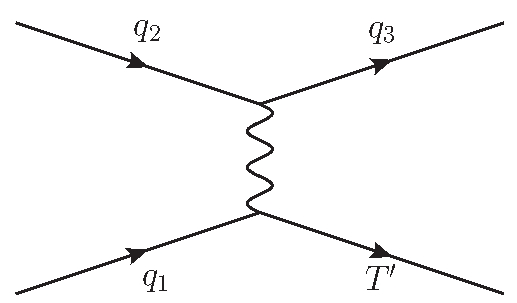
\includegraphics[width=0.9\textwidth]{../figs/Tchannel_T_single.jpg}\\
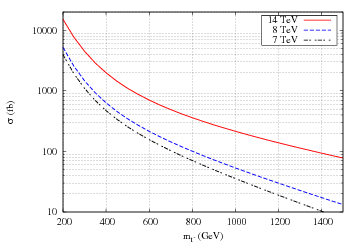
\includegraphics[width=1.0\textwidth]{../figs/pheno_prod_single_tp.png}
\end{center}
\end{column}
\end{columns}

\end{frame}

\begin{frame}{Datasets}
\vspace{-.2cm}

%\begin{table*}[htbH]
\begin{center}
\resizebox{\textwidth}{!}{
\begin{tabular}{|c|c|}
\hline 
Dataset name & Int. Luminosity ($\text{pb}^{-1}$) \\
\hline
/MultiJet/Run2012A-22Jan2013-v1/AOD & 889.4 \\
/MultiJet1Parked/Run2012B-05Nov2012-v2/AOD & 4429.0 \\
/MultiJet1Parked/Run2012C-part1-05Nov2012-v2/AOD & 494.6 \\
/MultiJet1Parked/Run2012C-part2-05Nov2012-v2/AOD & 6654.0 \\
/MultiJet1Parked/Run2012D-part1-10Dec2012-v1/AOD & 5955.1 \\
/MultiJet1Parked/Run2012D-part2-17Jan2013-v1/AOD & 734.0 \\
/MultiJet1Parked/Run2012D-part2-PixelRecover-17Jan2013-v1 & 538.4 \\
\hline
\multicolumn{1}{|r|}{\textit{Total}} & 19694.5 \\
\hline
\end{tabular}
}
%\caption{List of Multijet Primary Dataset used in the analysis and the corresponding integrated luminosity calculated using the golden JSON (Java Script Object Notation) file. The golden JSON file contains the information about the luminosity sections considered as good for all runs. A good luminosity section is defined as a luminosity section where the detector was fully functioning, this is all subsystems were taking data and without problems.  \label{tab:datasets}}
\end{center}
%\end{table*}

%\begin{table*}[htbH]
\begin{center}
\resizebox{\textwidth}{!}{
\begin{tabular}{|c|c|c|}
\hline 
Samples & Cross-Section (pb) & Number of events\\
\hline
QCD\_Pt-120to170\_TuneZ2star\_8TeV\_pythia6 & 16\(\times 10^4\) & 5.9M\\
QCD\_Pt-170to300\_TuneZ2star\_8TeV\_pythia6 & 34\(\times 10^3\) & 5.8M\\
QCD\_Pt-300to470\_TuneZ2star\_8TeV\_pythia6 & 18\(\times 10^2\) & 5.9M\\ 
QCD\_Pt-470to600\_TuneZ2star\_8TeV\_pythia6 & 114 & 3.9M\\
QCD\_Pt-600to800\_TuneZ2star\_8TeV\_pythia6 & 27 & 3.9M\\
QCD\_Pt-800to1000\_TuneZ2star\_8TeV\_pythia6 & 3.5 & 3.9M\\
QCD\_HT-500To1000\_TuneZ2star\_8TeV-madgraph-pythia6 & 84\(\times 10^2\) & 30M\\ 
QCD\_HT-1000ToInf\_TuneZ2star\_8TeV-madgraph-pythia6 & 2\(\times 10^2\) & 14M\\ 
TTJets\_MSDecays\_central\_TuneZ2star\_8TeV-madgraph-tauola & 247.7 [NNLO] & 62M\\
TprimeJetToTH\_\textbf{M-700}\_TuneZ2star\_8TeV-madgraph\_tauola & 143.7 & 99K \\
\hline
\end{tabular}
}
%\caption{List of Monte-Carlo background samples used in the analysis, their corresponding cross-section and their number of events.\label{tab:MCbkg}}
\end{center}
%\end{table*}

\tiny{Signal samples were done with $T'\to tH$ with $H\to\tau^{+}\tau^{-}$ (6\%) and $H\to b\bar{b}$ (94\%). Correction with weight of 0.61 to obtain correct $Br(H\to b\bar{b})=0.57$. }

\end{frame}

\begin{frame}{Event selection}
\vspace{-.2cm}

\begin{columns}

\begin{column}{.55\textwidth}
\begin{block}{Event processing}
\begin{itemize}\scriptsize
  \item Data processed using ``golden'' JSON file: Consider only validated lumi sections
  \item PAT processing
    \begin{itemize}\tiny
    \item Jets reconstructed with PF algorithm and CHS
    \item Jets: \ptg{20} and $|\eta|<5$
    \item At least one good primary vertex: $\text{n.d.o.f.} \ge 4,\; |z|<24 \;\text{cm},\; |\rho|< 2 \;\text{cm}$
    \item Global tag: Calibration and alignment info for data, MC corrected to get close to data conditions
    \end{itemize}
  \item Pile-up corrections: Simulated PU in MC was corrected to observed PU in Data
\end{itemize}
\end{block}
\end{column}

\begin{column}{.45\textwidth}
\vspace{-.9cm}
\begin{figure}[!Hhtbp]
  \begin{center}
    \includegraphics[width=1.0\textwidth]{../figs/Ana/Nvtcs.png}
  \end{center}
\end{figure}
\vspace{-.75cm}
\begin{block}{}
\tiny Number of vertices distribution for data and MC samples. The comparison has been performed after basic selection except number of b-tagged jets (the basic selection is described in the next slides). The gray band correspond to the statistical error of MC samples sum. Normalization of MC samples was done to the 19.7~fb$^{-1}$.
\end{block}
\end{column}

\end{columns}
\end{frame}

\begin{frame}{Basic selection}
\vspace{-.2cm}

\begin{block}{}
  \begin{itemize}\scriptsize
  \item Trigger L1: at least 4 central jets (\etal{3}) with \ptg{32}~or \ptg{36}~or \ptg{40} \\
                    or at least 2 central jets with \ptg{52}~or \ptg{56}~or \ptg{64} \\
                    or events with \HTg{125}~or \HTg{150}~or \HTg{175}
  \item HLT: 6 central jets with a \ptg{20}, 4 with a \ptg{60} and 2 with a \ptg{80}
  \item \textbf{First offline cut}: 2 jets with \ptg{90}, 2 jets with \ptg{70} and 2 jets with \ptg{30}
  \end{itemize}
\end{block}

\begin{columns}
\begin{column}{.50\textwidth}
\vspace{-.2cm}
\begin{block}{}
  \scriptsize \textbf{Second cut}: At least 5 jets with \ptg{30} and \etal{2.5} and at least one additional jet with \ptg{30} and \etal{5} were required
\end{block}

\vspace{-.2cm}
\begin{block}{}
\scriptsize \textbf{Figure}: Distribution of pseudorapidity of the accompanying jet produced with the \Tp. The distribution is taken from the signal MC sample with M=700 \GeVcc~and it is normalized to unity.
\end{block}
\end{column}

\begin{column}{.50\textwidth}
\vspace{-.2cm}
\begin{figure}[!Hhtbp]
  \begin{center}
    \includegraphics[width=1.0\textwidth]{../figs/Ana/SixthJetMCTruth.png}
    %\caption{Distribution of pseudorapidity of the accompanying jet produced with the \Tp. The distribution is taken from the signal MC sample with M=700 \GeVcc~and it is normalized to unity.}
    %\label{fig:SixthJetTp}
  \end{center}
\end{figure}
\end{column}
\end{columns}

\end{frame}

\begin{frame}{Basic selection}
\vspace{-.2cm}

\begin{columns}
\begin{column}{.50\textwidth}
\begin{block}{}
\scriptsize \textbf{3rd cut}: the leading jet was required to have a \ptg{150}
\end{block}
\vspace{-.2cm}
\begin{block}{}
\scriptsize \textbf{4th cut}: \HTg{550} was required
\end{block}
\vspace{-.2cm}
\begin{block}{}
\scriptsize \textbf{Figure}: Distribution of the $H_{T}$ variable for data and the sum of the MC samples normalized to luminosity. The signal sample (M=700 \GeVcc) is over-imposed on top of the stack of the MC samples. The gray band represents the statistical uncertainties from the sum of the MC background. Reasonable agreement is observed, with the multijet process as the dominant process at this stage. Normalization of samples was done to luminosity.
\end{block}
\end{column}

\begin{column}{.50\textwidth}
\begin{figure}[!Hhtbp]
  \begin{center}
    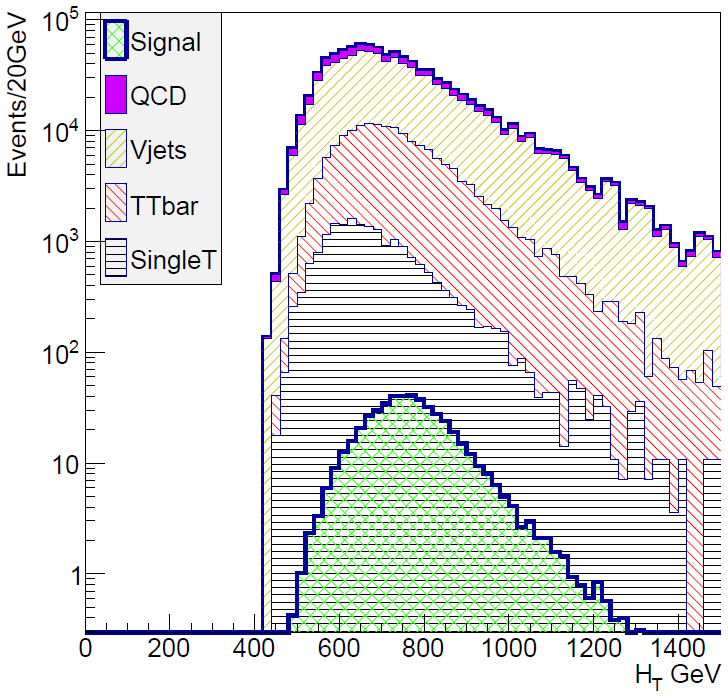
\includegraphics[width=1.0\textwidth]{../figs/Ana/HT.png}
    %\caption{Distribution of the $H_{T}$ variable for data and the sum of the MC samples normalized to luminosity. The signal sample (M=700 \GeVcc) is over-imposed on top of the stack of the MC samples. The gray band represents the statistical uncertainties from the sum of the MC background. Reasonable agreement is observed, with the multijet process as the dominant process at this stage. Normalization of samples was done to luminosity.}
    %\label{fig:HT}
  \end{center}
\end{figure}
\end{column}

\end{columns}
\end{frame}